\documentclass{article}
\usepackage[rightcaption]{sidecap}
\usepackage{graphicx} % Required for inserting images
\usepackage{multirow}
\usepackage[top=4cm, bottom=4cm, left=3cm, right=3cm]{geometry}
\usepackage[labelfont=bf, justification=raggedright, singlelinecheck=false]{caption}
\usepackage[european, americanvoltages]{circuitikz} % Per i circuiti
\usepackage{pgfplots}
\pgfplotsset{compat=1.18} % Ottimizza la compatibilità di PGFPlots
\usepgfplotslibrary{groupplots} % Consente di allineare modulo e fase
\newcommand\tab[1][1cm]{\hspace*{#1}}
\usepackage[T1]{fontenc}
\usepackage{appendix}
\usepackage{tabularx}
\usepackage{float}
\usepackage{tcolorbox}
\usepackage{amsmath}
\usepackage{amssymb}
\usepackage{eso-pic} % for \BgThispage
\usepackage{tikz}
\usepackage{titlesec}
\usepackage{tocloft}
\usetikzlibrary{arrows.meta}
\usepackage[pages=some]{background}
\usepackage[italian]{babel}
\usepackage[colorlinks=true, linkcolor=black, citecolor=black, filecolor=black, urlcolor=blue]{hyperref}
\addto\captionsitalian{\renewcommand{\contentsname}{Indice}}
\backgroundsetup{scale=1.5,anchor=right,angle=0,opacity=0.1,contents={
\includegraphics[scale=1]{Misc/logo_standard (1).png}}}

% FORMATTAZIONE SOTTOTITOLI
%-----------------------------------------------------------
\titleformat{\subsection}
{\normalfont\Large\bfseries}{\thesubsection}{1em}{}

\titleformat{\section}
{\normalfont\Large\bfseries}{\thesection}{1em}{}
%-----------------------------------------------------------

% FORMATTAZIONE INDICE
%-----------------------------------------------------------
\renewcommand{\cftsecfont}{\normalfont\Large\bfseries}
\renewcommand{\cftsecpagefont}{\normalfont\Large\bfseries}

\renewcommand{\cftsubsecfont}{\normalfont\Large}
\renewcommand{\cftsubsecpagefont}{\normalfont\Large}

\setlength{\cftbeforesecskip}{0.5cm} 
\setlength{\cftbeforesubsecskip}{0.3cm}
%-----------------------------------------------------------

% TITOLO
%-----------------------------------------------------------
\title{
    Relazione : Amplificatori Operazionali e Filtri RC \\ 
    \vspace{0.3cm} 
    \Large Gruppo 03
}
%-----------------------------------------------------------

% AUTORI
%-----------------------------------------------------------
\author{
  Lorenzo Allocco \\ -- Mat. 061270XXXX
  \\ \\
  Riccardo La Porta \\ -- Mat. 0612709691
  \\ \\
  Francesco Grimaldi \\ -- Mat. 0612708839
  \\ \\
  Alessandro Altieri \\ -- Mat. 0612709239
}

\date{5 Giugno 2026}

\begin{document}
\BgThispage

\AddToShipoutPictureBG*{
  \begin{tikzpicture}[remember picture, overlay]
    \node [anchor=north west, inner sep=30pt] at (current page.north west)
      {
\includegraphics[height=1.5cm]{Misc/diem (1).png}};
    \node [anchor=center, opacity=0.05] at (current page.east)
      {
\includegraphics[scale=1.5]{Misc/logo_standard (1).png}};
  \end{tikzpicture}
}
%-----------------------------------------------------------

\maketitle

% INDICE
%-----------------------------------------------------------
\newpage
\tableofcontents
\newpage
%-----------------------------------------------------------

\section{Obiettivi dell'esperienza}
    La seguente relazione si pone come obiettivo quello di descrivere l'esperienza di laboratorio tenutasi
    nell'ambito del corso di Tecnologie Elettriche per l'Informatica Industriale.\\ \\
    Lo scopo è quello di introdurre lo studente all'utilizzo e alla comprensione dell'Oscilloscopio (Hantek 6022BL) come strumento di misura, nonchè
    comprendere la sua applicazione nello studio e nell'analisi di segnali elettrici.
    \\
    \\
    L'attività pratica di laboratorio si suddivide in 4 fasi:
    \
    \begin{itemize}
        \item Configurazione dello strumento
        \item Misura del segnale di calibrazione
        \item Calibrazione dello strumento
        \item Compensazione capacitiva della sonda
    \end{itemize}
\newpage

\section{Introduzione e cenni teorici}
    La calibrazione dell'oscilloscopio, e in particolare la compensazione capacitiva della sonda,
    sono procedure fondamentali per garantire la fedeltà e l'accuratezza delle misure nel dominio del tempo
    e della frequenza. Una sonda passiva attenuata (tipicamente di tipo 10X) non si comporta come un conduttore
    ideale: il suo modello equivalente è un partitore resistivo-capacitivo, composto dalla resistenza e dalla
    capacità della sonda stessa in serie, che si interfaccia con l'impedenza d'ingresso dell'oscilloscopio
    (tipicamente $1\text{M}\Omega$  in parallelo a una capacità parassita). Il cavo coassiale della sonda introduce
    a sua volta una capacità distribuita che si somma a quella parassita dell'ingresso. Per garantire una risposta
    in frequenza piatta è necessario che le costanti di tempo dei due rami del partitore siano uguali:

    \begin{equation*}
        \boxed{R_{sonda} \cdot C_{sonda} = R_{in} \cdot C_{in}}
    \end{equation*}

    \noindent Se questa condizione non è soddisfatta, il sistema si comporta come un filtro: le componenti ad alta frequenza
    vengono attenuate (sonda sottocompensata) oppure amplificate (sonda sovracompensata), introducendo distorsione
    nella forma d'onda visualizzata. La compensazione si realizza agendo su un condensatore variabile (trimmer capacitivo)
    integrato nel corpo della sonda. Il segnale di riferimento utilizzato per questa operazione è un'onda quadra a frequenza
    nota generata internamente dall'oscilloscopio: poiché un'onda quadra contiene ricche componenti armoniche ad alta frequenza,
    eventuali errori di compensazione si manifestano chiaramente come deformazioni sui fronti di salita e di discesa.
    \\

    % === MODELLO EQUIVALENTE SONDA E OSCILLOSCOPIO ===
    \begin{figure}[H]
        \centering
        \begin{circuitikz}[scale=1.1, transform shape]
            % --- GENERATORE DI CALIBRAZIONE ONDA QUADRA ---
            \draw (0,0) to[vsource, l=$V_{gen}$] (0,2.5) -- (1,2.5);
            
            % --- BLOCCO RAMO 1: SONDA (ATTENUATORE 10X) ---
            \draw (1,2.5) -- (2.5,2.5)
                to[R, l=$R_{sonda}$, o-o] (4.5,2.5);
            \draw (1,2.5) -- (1,4) 
                to[vC, l=$C_{sonda}$] (4.5,4) -- (4.5,2.5);
                
            % Delimitazione visiva del blocco Sonda
            \draw[dashed, gray] (1.8, 4.9) rectangle (4.9, 1.6);
            \node[text=gray, font=\small\bfseries] at (3.35, 1.8) {Sonda Passiva};

            % Nodo di collegamento tra Sonda e Ingresso
            \draw (4.5,2.5) -- (6.5,2.5) node[circle, fill, inner sep=1.5pt] (nodoV) {};
            
            % --- BLOCCO RAMO 2: INGRESSO OSCILLOSCOPIO ---
            \draw (6.5,2.5) -- (6.5,2)
                to[R, l=$R_{in}$] (6.5,0);
            \draw (6.5,2.5) -- (8,2.5) -- (8,2)
                to[C, l=$C_{in}$] (8,0) -- (6.5,0);
                
            % Delimitazione visiva del blocco Oscilloscopio
            \draw[dashed, gray] (5.4, 3.5) rectangle (9.2, -0.8);
            \node[text=gray, font=\small\bfseries] at (7.25, -0.6) {Ingresso Oscilloscopio};

            % --- MORSETTI DI LETTURA CANALE ---
            \draw (8,2.5) -- (9.5,2.5) to[short, -o] (10,2.5) node[above] {$V_{ch}$};
            
            % --- LINEA DI MASSA COMUNE ---
            \draw (10,0) to[short, o-] (0,0) node[ground] {};
            \draw (6.5,0) node[circle, fill, inner sep=1.5pt] {};
            
        \end{circuitikz}

        \captionsetup{justification=centering, singlelinecheck=false, font=small}
        \caption{Schema circuitale equivalente del sistema sonda-oscilloscopio.}
        \label{fig:modello_sonda_oscilloscopio}
    \end{figure}

\newpage

\section{Strumentazione e Componenti}
    La strumentazione utilizzata durante l'esperienza è elencata nella tabella seguente:

    \begin{table}[H]
        \centering
        
        \begin{tabularx}{\textwidth}{|X|X|X|}
            \hline
            \textbf{Strumento} & \textbf{Modello} & \textbf{Caratteristiche} \\ \hline
            Oscilloscopio Digitale & Hantek 6022BL & 2 canali, 20 MHz, 48 MS/s \\ \hline
            Generatore di Funzioni per la calibrazione & Hantek 6022BL & Integrato nello strumento \\ \hline
            Software & DPO & Software per macchine Windows \\ \hline
            Software & OpenHantek & Software open source disponibile su macchine linux \\ \hline
        \end{tabularx}
    \caption{Specifiche della strumentazione di laboratorio.}
    \end{table}

\section{Schema del Circuito e Procedura Sperimentale}

\subsection{Compensazione della sonda}

    Il setup sperimentale per questa fase prevede il collegamento diretto tra il generatore
    del segnale di calibrazione integrato nello strumento e l'ingresso del canale 1 (CH1)
    dell'oscilloscopio tramite la sonda in esame. La procedura si svolge nei seguenti passi: \\ \\

    \noindent \textbf{Configurazione iniziale dello strumento}: avviare il software, verificare la corretta rilevazione
    dello strumento e impostare la scala temporale a 1 ms/div e quella verticale a 2 V/div. La situazione iniziale,
    con sonda non ottimizzata, è riportata in Figura 2. \\ \\ 
    
    \noindent \textbf{Collegamento della sonda al segnale di calibrazione}: agganciare la punta della sonda al connettore di
    calibrazione dell'oscilloscopio. \\ \\

    \noindent \textbf{Osservazione e regolazione}: analizzare la forma d'onda e agire sul trimmer capacitivo della sonda. Tre
    condizioni sono possibili:
    
    \begin{itemize}
        \item fronti verticali e livelli stabili: sonda correttamente compensata;
        \item fronti arrotondati: sonda sottocompensata, aumentare il valore del trimmer;
        \item picchi di overshoot sui fronti: sonda sovracompensata, ridurre il valore del trimmer.
    \end{itemize}

    \noindent \textbf{Verifica finale}: una volta raggiunta la compensazione ottimale, i due canali mostrano parametri coerenti tra loro. Come si osserva in Figura 3 , entrambi i canali presentano
    $f = 2.000\,\mathrm{kHz}$,
    $V_{pp} \approx 3.5\,\mathrm{V}$
    $T = 500\,\mu\mathrm{s}$,
    confermando la corretta calibrazione della sonda.

\newpage

\section{Raccolta e Analisi dei Dati Sperimentali}
    Le acquisizioni effettuate durante la sessione di laboratorio documentano l'evoluzione della misura nelle diverse fasi della procedura. 

    \begin{figure}[H]
    \centering
    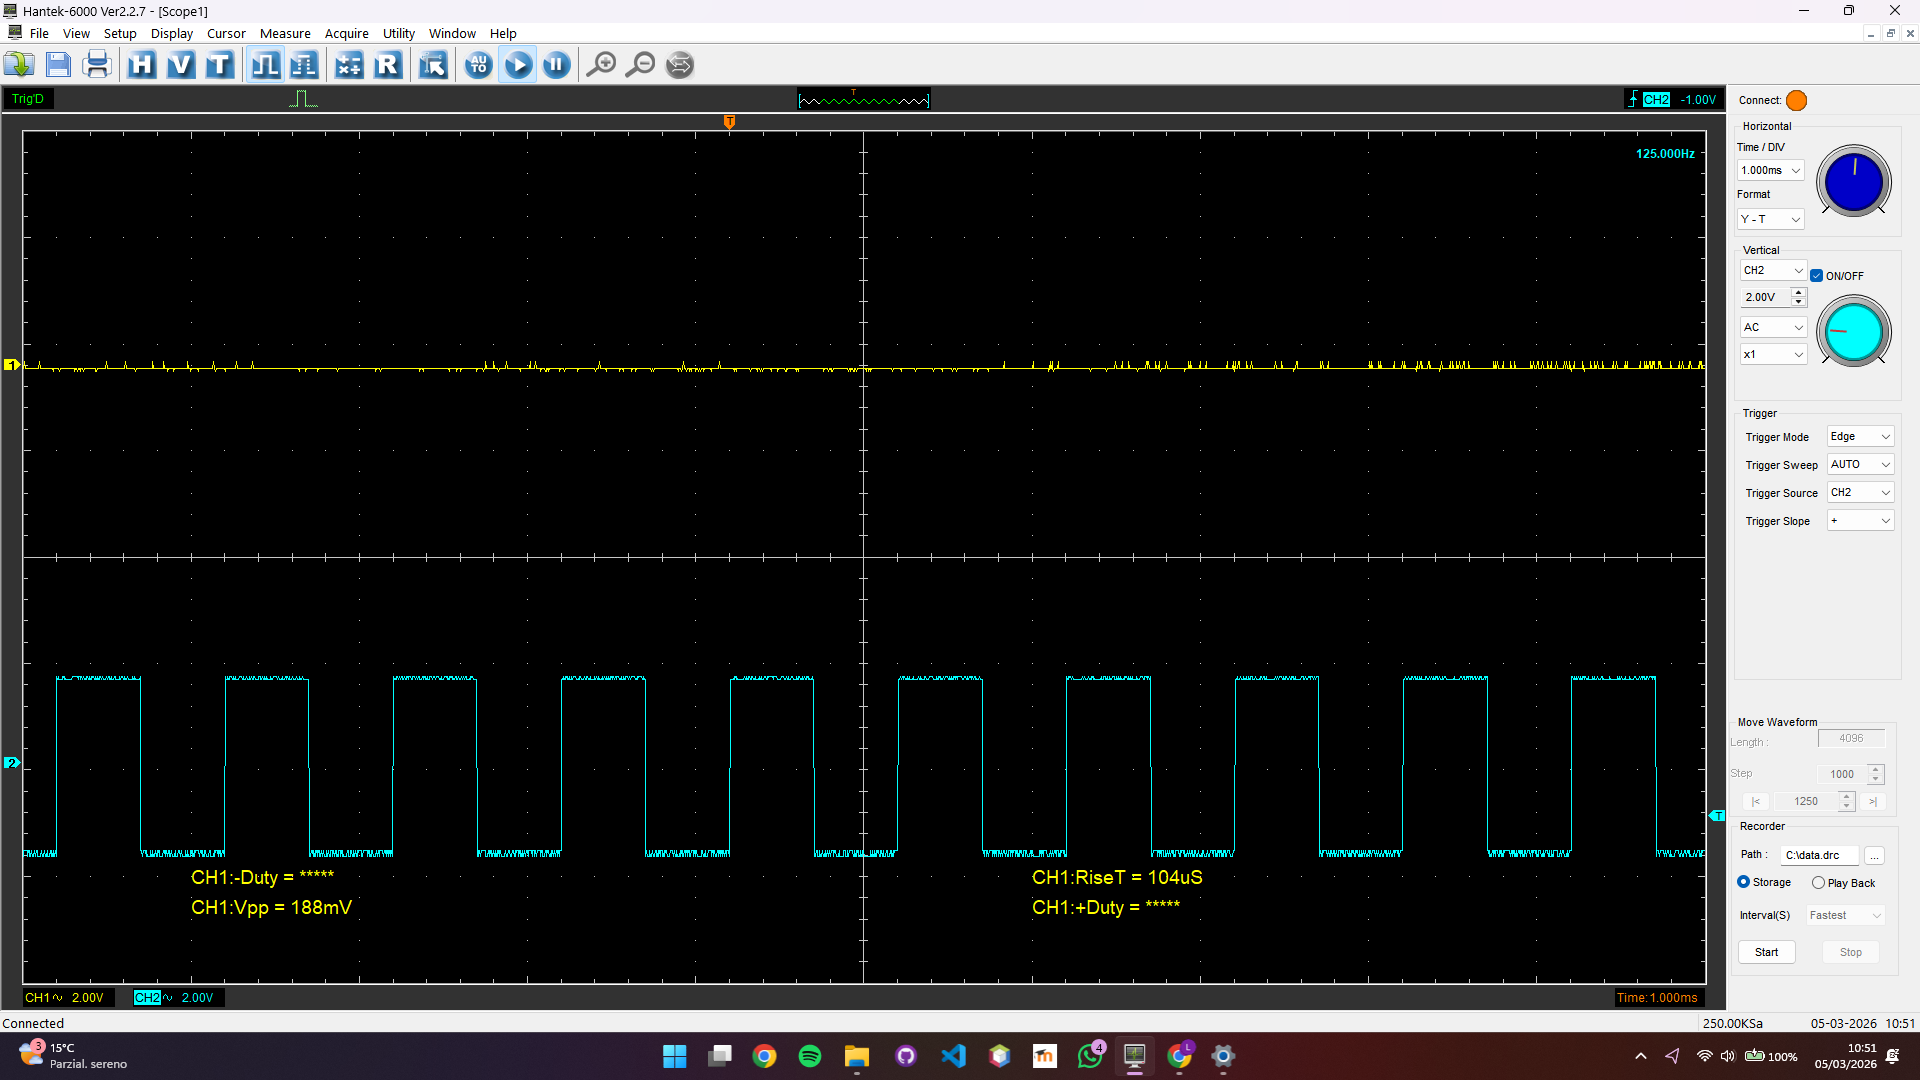
\includegraphics[width=0.5\textwidth]{immagini/Figura1.png}
    \caption{ Configurazione iniziale: CH1 con segnale a bassa ampiezza (Vpp = 188 mV, RiseT = 104 µs). Scala 1 ms/div, trigger su CH2.}
    \end{figure}

    \begin{figure}[H]
    \centering
    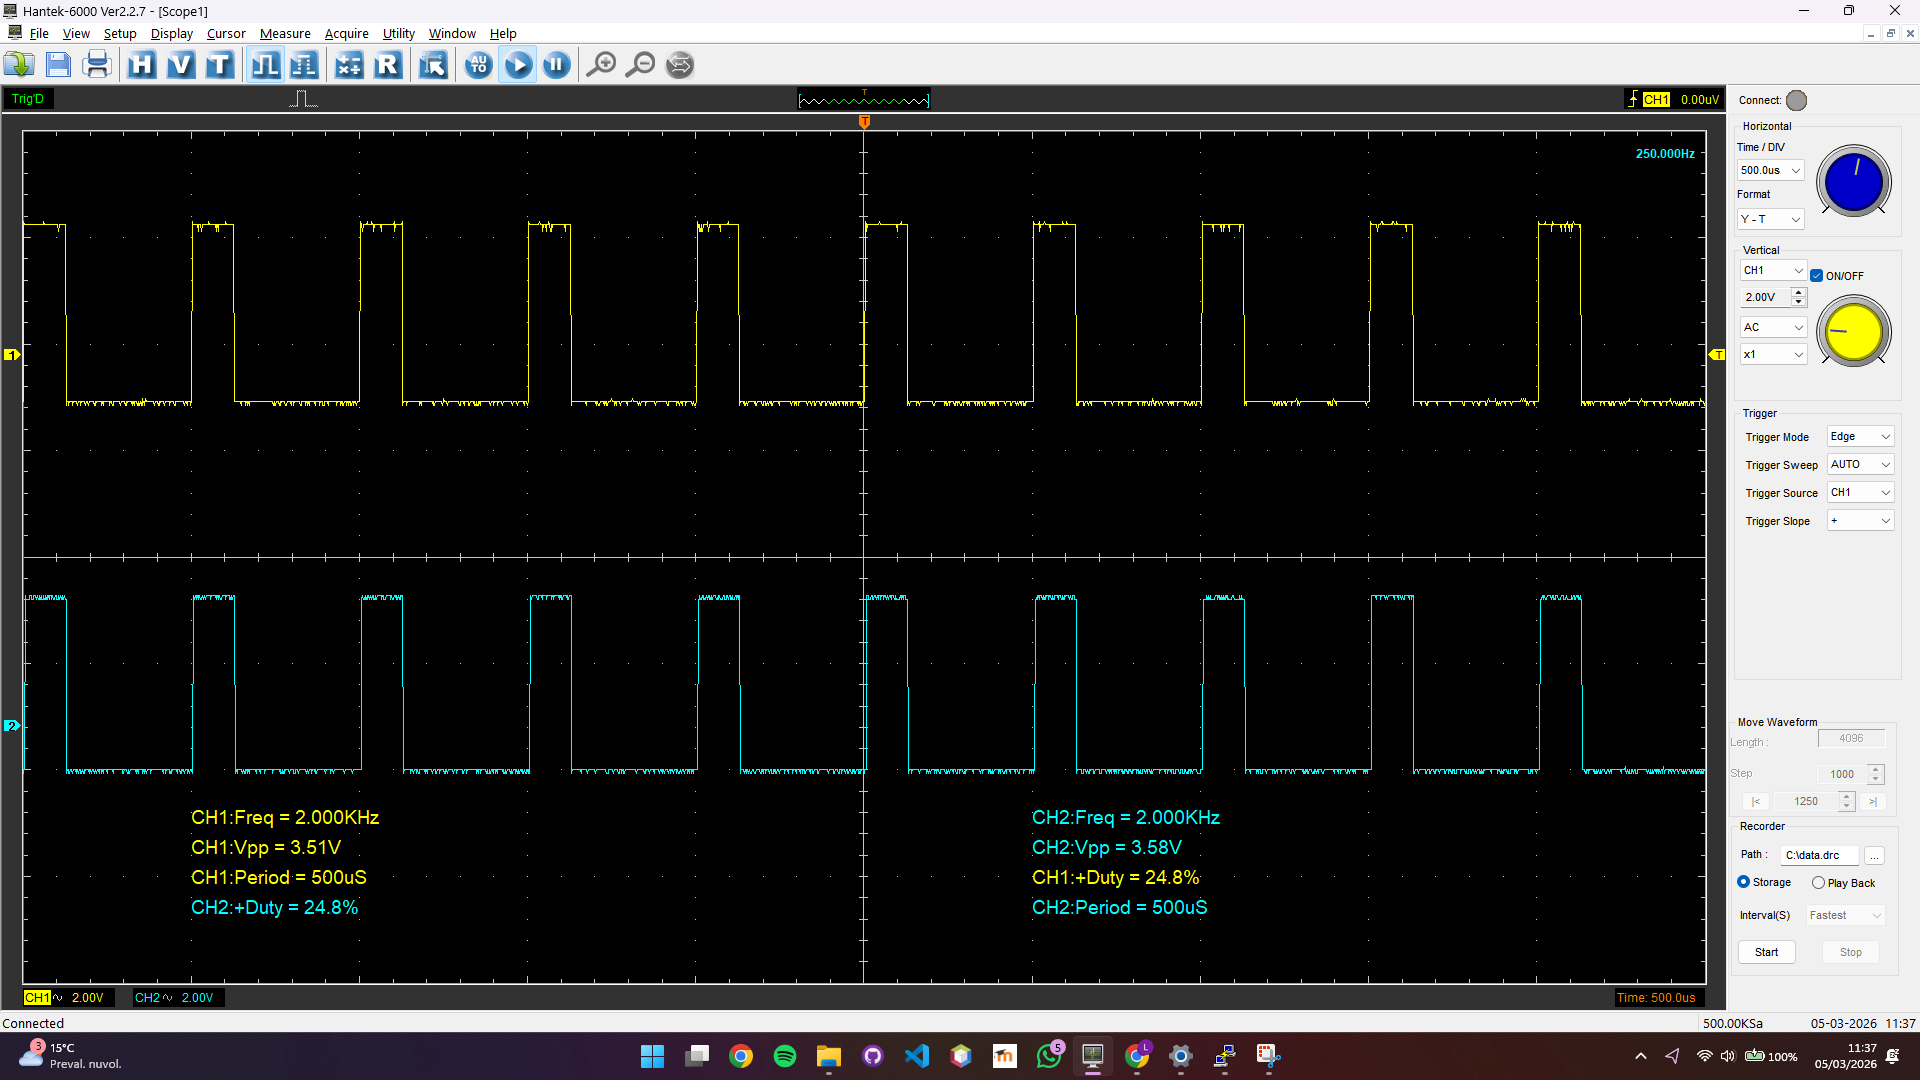
\includegraphics[width=0.5\textwidth]{immagini/Figura4.png}
    \caption{ ( Stato finale dopo calibrazione: entrambi i canali a f = 2.000 kHz, $V_{pp} \approx 3.5\,\mathrm{V}$, T = 500 µs, duty cycle 24.8\%, Scala 500 µs/div.)}
    \end{figure}
     
\newpage

\section{Discussione dei Risultati}
I risultati ottenuti sono in accordo con quanto previsto dalla teoria. La compensazione capacitiva della sonda ha un impatto
diretto sulla fedeltà della misura: una sonda non correttamente compensata introduce un errore sistematico che dipende dalla
frequenza del segnale, rendendo inaffidabili le misure su segnali con componenti ad alta frequenza. \\

\noindent In particolare, la condizione di sottocompensazione è critica in tutte le applicazioni in cui è necessario misurare con
precisione i tempi di salita e di discesa di un segnale digitale o impulsivo. Una lettura distorta del fronte potrebbe portare
a una sovrastima del tempo di salita reale, con conseguenti errori nella caratterizzazione di circuiti digitali o nella misura
della banda del segnale. \\

\noindent La condizione di sovracompensazione, seppur meno comune in pratica, può indurre a ritenere presente
un overshoot nel segnale anche quando questo non esiste nel circuito reale, con possibili errori di interpretazione nella valutazione
della stabilità di un sistema. \\

\noindent I dati rilevati mostrano che nella fase finale (Figura 3) i due canali presentano valori molto vicini tra loro
(differenza di Vpp < 2\%), confermando la riuscita della procedura di calibrazione e la coerenza delle misure tra i canali dello strumento.

\section{Conclusioni}
L'esperienza di laboratorio ha permesso di acquisire familiarità con l'oscilloscopio digitale Hantek 6022BL e con le procedure di base necessarie per un corretto utilizzo dello strumento.
La compensazione capacitiva della sonda, pur essendo un'operazione semplice e rapida, si è rivelata fondamentale per garantire l'affidabilità delle misure. Essa rappresenta un prerequisito necessario prima di qualsiasi sessione di misura, specialmente quando si lavora con segnali ad alta frequenza o con forme d'onda impulsive.
I concetti appresi costituiscono una base teorica e pratica utile per tutte le successive esperienze di laboratorio del corso di Tecnologie Elettriche per l'Informatica Industriale.

\newpage

\end{document}